% use xelatex to compile the document. 

\documentclass[sublist,a4paper,twoside,11pt]{article}
\usepackage[utf8]{inputenc}
\usepackage{a4wide}
%%% Various other
\usepackage{hyperref}
\hypersetup{
	colorlinks=true,
	linkcolor=blue,
	filecolor=magenta,      
	urlcolor=cyan,
}

\urlstyle{same}

\usepackage{amsmath}
\usepackage{breqn}
\usepackage{amssymb}
\usepackage{tabularx}
\usepackage{xltxtra}
%\usepackage{xgreek}
\usepackage{graphicx}

\usepackage{amsthm}

\author{André de Souza Mendes, N. Papadakis}
\title{Simple vehicle model 4dof }

\makeindex

% \makeglossaries

\begin{document}

\maketitle

\tableofcontents

% \begin{folhaderosto}
% Dissertação de Mestrado apresentada ao Centro Universitário da FEI para obtenção do título de Mestre em Engenharia Mecânica, orientado pelo Prof. Dr. Agenor de Toledo Fleury.
% \end{folhaderosto}

% \fichacatalografica						% procura o arquivo "ficha.pdf"
% \folhadeaprovacao						% procura o arquivo "ata.pdf"

% \dedicatoria{À minha família.}

% \begin{agradecimentos}
% Obrigado
% \end{agradecimentos}

% \epigrafe{Science is more than a body of knowledge, it's a way of thinking. A way of skeptically interrogating the universe with a fine understanding of human fallibility.}{Carl Sagan}

% \begin{resumo}
% resumo
% \palavraschave{Dinâmica veicular. Veículos articulados. Análise de estabilidade. Trajetórias de fase. Expoentes de Lyapunov.}
% \end{resumo}

% \begin{abstract}
% abstract
% \keywords{Vehicle dynamics. Articulated vehicles. Stability analysis. Phase trajectories. Lyapunov exponents.}
% \end{abstract}

% {
% 	\pagestyle{empty}
% 	\listoffigures
% 	\listoftables
% %	\listofalgorithms
%     \printglossaries
%     % \glsaddall
%     \tableofcontents
% }




\section{Articulated Vehicle Model}

The physical model of the set is illustrated in the figure \ref{modelSimple}. In order to characterize the dynamics of this system we use the base \( \Omega_{\rm O} = \{ {\rm O} {\bf i} {\bf j} {\bf k} \}\) fixed in the inertial frame .

The base  \( \Omega_{\rm T} = \{ {\rm T} {\bf t}_x {\bf t}_y {\bf t}_z \}\)  is attached to the tractor truck and base \( \Omega_{\rm S} = \{ {\rm S} {\bf s}_x {\bf s}_y {\bf s}_z \}\)  is attached to the semi-trailer. The unit vectors  \({\bf t}_x\) and \({\bf s}_x\) point forward in the longitudinal direction of both modules and the verses \({\bf t}_y\) e \({\bf s}_y\) point to the left. 

To assist in the description of the magnitudes on the front axle, the base \( \Omega_{\rm F} = \{ {\rm F} {\bf e}_x {\bf e}_y {\bf e}_z \}\)  is defined with respect to the front axle with the vector  \({\bf e}_x\) pointing forward in the longitudinal direction of the tire and \({\bf e}_y\) pointing to the left.

The points  \({\rm T}\) and \({\rm S}\)  define the center of mass of the tractor-truck and the semi-trailer, respectively. \({\rm F}\) and \({\rm R}\) locate the front and rear axles, respectively. \({\rm A}\)  is the point of articulation and \({\rm M}\) is the axis of the semi-trailer.

The point \({\rm O}\) is the origin of the system and is fixed in the inertial frame. The distance \(a\) separates the points \({\rm F}\) and \({\rm T}\)  and the distance  \(b\) separates the points \({\rm T}\) and \({\rm R}\) .  \(c\) separates points \({\rm R}\) and \({\rm A}\), \(d\) separates points \({\rm A}\) e \({\rm S}\) and  \(e\) separates points \({\rm S}\) e \({\rm M}\). 


The velocity vectors  \({\bf v}\)  and the drift angles \(\alpha\) receive the subscripts referring to the points to which they are associated.
	
The modeling of the tractor-trailer and semi-trailer consists of the use of two rigid bodies that move on a horizontal plane and are joined by a point of articulation. In this way, the model has four degrees of freedom. Therefore, generalized coordinates can be given by

\begin{subequations}
\begin{equation}
    q_1 = x
\end{equation}
\begin{equation}
    q_2 = y
\end{equation}
\begin{equation}
    q_3 = \psi
\end{equation}
\begin{equation}
    q_4 = \phi,
\end{equation}
\end{subequations}

where \(x \) and \(y \) are the longitudinal and transverse coordinates of the center of mass of the tractor-truck, respectively. \(\psi \) is the absolute orientation angle of the tractor-trailer and \(\phi \) is the relative orientation angle of the semi-trailer.

\begin{figure}[h]
	\centering
	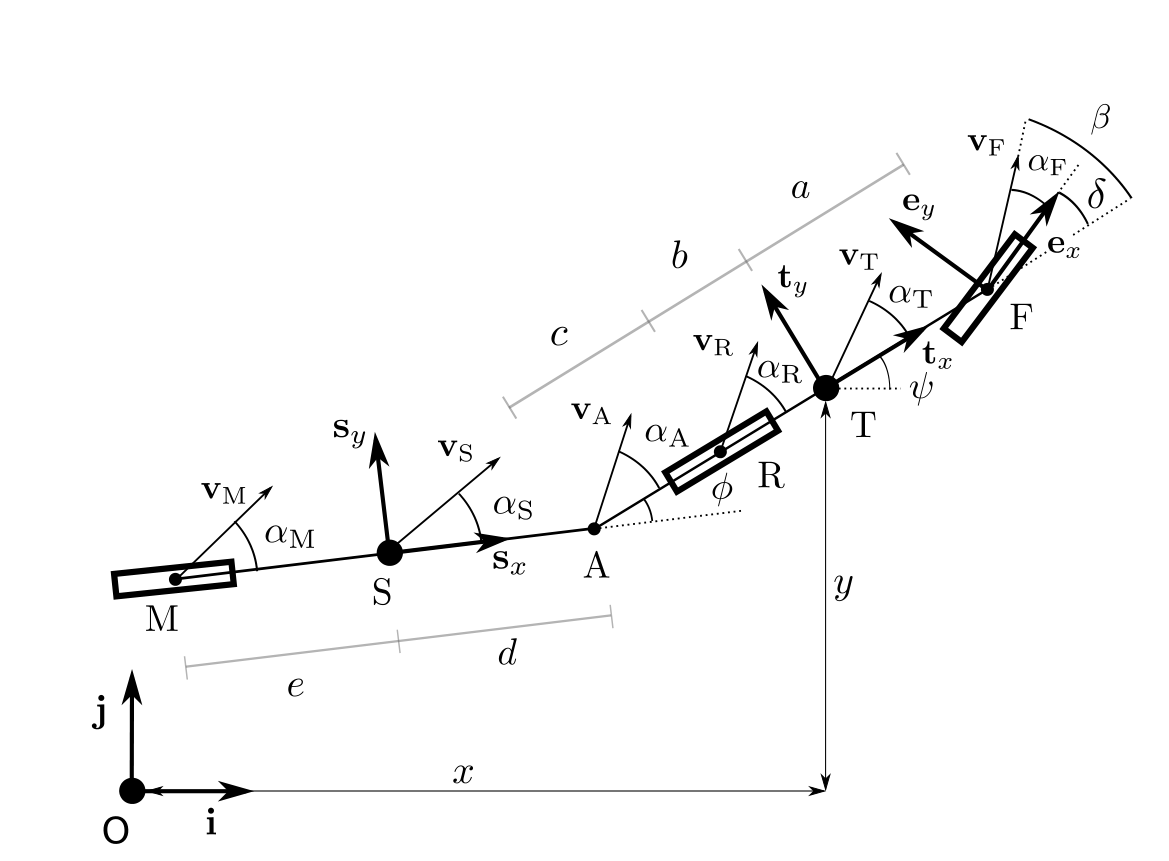
\includegraphics[width=0.7\linewidth]{figures/SingeTrackBicycleModel}
    \caption{Single track bicycle model.}	\label{fig:singetrackbicyclemodel}
\end{figure}



\subsection{Nonlinear Model}

The vector position of the tractor-truck center-of-mass in relation to the point \(O \) is

\begin{equation} \label{positionTractor}
    {\bf p}_{{\rm T}/{\rm O}} = x {\bf i} + y {\bf j}.
\end{equation}

The position vector of the center of mass of the semi-trailer is

\begin{equation} \label{positionSemitrailer}
    {\bf p}_{{\rm S}/{\rm O}} = \left[ x - \left( b + c \right) \cos \psi - d \cos \left( \psi - \phi \right) \right] {\bf i} + \left[ y - \left( b + c \right) \sin \psi - d \sin \left( \psi - \phi \right) \right] {\bf j}.
\end{equation}

Differentiating the equation \eqref {positionTractor} with respect to time we have

\begin{equation} \label{velocityTractor}
    {\bf v}_{\rm T} = \dot{x} {\bf i} + \dot{y} {\bf j}.
\end{equation}

Deriving the equation \eqref {positionSemitrailer} with respect to time we have

\begin{eqnarray} \label{velocitySemitrailer}
    \nonumber
    {\bf v}_{\rm S} &=& \left[ \dot{x} + \left( b + c \right) \dot{\psi} \sin \psi + d \left( \dot{\psi} - \dot{\phi} \right) \sin \left( \psi - \phi \right) \right] {\bf i} + ... \\
    \nonumber
     ... &+& \left[ \dot{y} - \left( b + c \right) \dot{\psi} \cos \psi - d \left( \dot{\psi} - \dot{\phi} \right) \cos \left( \psi - \phi \right) \right] {\bf j}. \\
\end{eqnarray}


The angular velocity vector of the tractor-truck is:

\begin{equation} \label{angulaVelTrailer}
    {\bf w}_T = \dot{\psi} {\bf k}.
\end{equation}

The angular velocity vector of the semi-trailer is

\begin{equation} \label{angulaVelSemir}
    {\bf w}_S = \left( \dot{\psi} - \dot{\phi} \right) {\bf k}
\end{equation}

The kinetic energy of the system is:

\begin{equation} \label{kinEnergyGeneral}
    T = \frac{1}{2} m_{T} {\bf v}_{\rm T} \cdot {\bf v}_{\rm T} + \frac{1}{2} m_{S} {\bf v}_{\rm S} \cdot {\bf v}_{\rm S} + \frac{1}{2} \left\{ {\bf w}_T \right\}^T \left[ {\bf J}_T \right] \left\{ {\bf w}_T \right\} + \frac{1}{2} \left\{ {\bf w}_S \right\}^T \left[ {\bf J}_S \right] \left\{ {\bf w}_S \right\}.
\end{equation}

Substituting the equations \eqref {velocityTractor}, \eqref {velocitySemitrailer}, \eqref {angulaVelTrailer}, \eqref {angulaVelSemir} in \eqref {kinEnergyGeneral}

\begin{equation} \label{kinEnergyCoord}
    T = \frac{1}{2} m_{T} \left( \dot{x}^2 + \dot{y}^2 \right) + \frac{1}{2} m_{S} \left( C_1^2 + C_2^2 \right) + \frac{1}{2} I_{T} \dot{\psi}^2 + \frac{1}{2} I_{S} \left( \dot{\psi} - \dot{\psi} \right)^2,
\end{equation}

where 

\begin{subequations} \label{constants}
\begin{equation}
    C_1 = \dot{x} + \left( b + c \right) \dot{\psi} \sin \psi + d \left( \dot{\psi} - \dot{\phi} \right) \sin \left( \psi - \phi \right)
\end{equation}
\begin{equation}
    C_2 = \dot{y} - \left( b + c \right) \dot{\psi} \cos \psi - d \left( \dot{\psi} - \dot{\phi} \right) \cos \left( \psi - \phi \right).
\end{equation}
\end{subequations}

Deriving the equation \eqref {constants} we have

\begin{subequations} \label{constantsTimeDiff}
\begin{equation}
    \dot{C}_1 = \ddot{x} + \left( b + c \right) \ddot{\psi} \sin \psi + \left( b + c \right) \dot{\psi}^2 \cos \psi + d \left( \ddot{\psi} - \ddot{\phi} \right) \sin \left( \psi - \phi \right) + d \left( \dot{\psi} - \dot{\phi} \right)^2 \cos \left( \psi - \phi \right)
\end{equation}
\begin{equation}
    \dot{C}_2 = \ddot{y} - \left( b + c \right) \ddot{\psi} \cos \psi + \left( b + c \right) \dot{\psi}^2 \sin \psi - d \left( \ddot{\psi} - \ddot{\phi} \right) \cos \left( \psi - \phi \right) + d \left( \dot{\psi} - \dot{\phi} \right)^2 \sin \left( \psi - \phi \right)
\end{equation}
\end{subequations}

The partial derivatives of the system's kinetic energy  (equation \eqref {kinEnergyCoord}) with respect to the generalized coordinates are:

\begin{subequations} \label{lagrangePartialTerm}
\begin{equation}
    \frac{\partial T}{\partial q_1} = \frac{\partial T}{\partial x} = 0
\end{equation}
\begin{equation}
    \frac{\partial T}{\partial q_2} = \frac{\partial T}{\partial y} = 0
\end{equation}
\begin{eqnarray}
    \nonumber
    \frac{\partial T}{\partial q_3} = \frac{\partial T}{\partial \psi} &=& m_S C_1 \left[ \left( b + c \right) \dot{\psi} \cos \psi + d \left( \dot{\psi} - \dot{\phi} \right) \cos \left( \psi - \phi \right) \right] + ... \\
    \nonumber
    ... &+& m_S C_2 \left[ \left( b + c \right) \dot{\psi} \sin \psi + d \left( \dot{\psi} - \dot{\phi} \right) \sin \left( \psi - \phi \right) \right] \\
\end{eqnarray}
\begin{equation}
    \frac{\partial T}{\partial q_4} = \frac{\partial T}{\partial \phi} = m_S C_1 \left[ - d \left( \dot{\psi} - \dot{\phi} \right) \cos \left( \psi - \phi \right) \right] + m_S C_2 \left[ - d \left( \dot{\psi} - \dot{\phi} \right) \sin \left( \psi - \phi \right) \right].
\end{equation}
\end{subequations}

The partial derivatives of the kinetic energy of the system in relation to the temporal derivatives of the generalized coordinates are:

\begin{subequations} \label{partialDiff}
\begin{equation}
    \frac{\partial T}{\partial \dot{q}_1} = \frac{\partial T}{\partial \dot{x}} = m_{T} \dot{x} + m_S C_1
\end{equation}
\begin{equation}
    \frac{\partial T}{\partial \dot{q}_2} = \frac{\partial T}{\partial \dot{y}} = m_{T} \dot{y} + m_S C_2
\end{equation}
\begin{eqnarray}
    \nonumber
    \frac{\partial T}{\partial q_3} = \frac{\partial T}{\partial \dot{\psi}} &=& m_S C_1 \left[ \left( b + c \right) \sin \psi + d \sin \left( \psi - \phi \right) \right] + ... \\
    \nonumber
    ... &+& m_S C_2 \left[ - \left( b + c \right) \cos \psi - d \cos \left( \psi - \phi \right) \right] + I_T \dot{\psi} + I_S \left( \dot{\psi} - \dot{\phi} \right) \\
\end{eqnarray}
\begin{equation}
    \frac{\partial T}{\partial q_4} = \frac{\partial T}{\partial \dot{\phi}} = m_S C_1 \left[ - d \sin \left( \psi - \phi \right) \right] + m_S C_2 \left[ d \cos \left( \psi - \phi \right) \right] - I_S \left( \dot{\psi} - \dot{\phi} \right).
\end{equation}
\end{subequations}

Deriving the equations \eqref{partialDiff} with respect to time we have

\begin{subequations} \label{lagrangeTimeTerm}
\begin{equation}
    \frac{d}{dt} \left( \frac{\partial T}{\partial \dot{q}_1} \right) = \frac{d}{dt} \left( \frac{\partial T}{\partial \dot{x}} \right) = m_{T} \ddot{x} + m_S \dot{C}_1
\end{equation}
\begin{equation}
    \frac{d}{dt} \left( \frac{\partial T}{\partial \dot{q}_2} \right) = \frac{d}{dt} \left( \frac{\partial T}{\partial \dot{y}} \right) = m_{T} \ddot{y} + m_S \dot{C}_2
\end{equation}
\begin{eqnarray}
    \nonumber
    \frac{d}{dt} \left( \frac{\partial T}{\partial \dot{q}_3} \right) = \frac{d}{dt} \left( \frac{\partial T}{\partial \dot{\psi}} \right) &=& m_S \dot{C}_1 \left[ \left( b + c \right) \sin \psi + d \sin \left( \psi - \phi \right) \right] + ... \\
    \nonumber
    ... &+& m_S C_1 \left[ \left( b + c \right) \dot{\psi} \cos \psi + d \left( \dot{\psi} - \dot{\phi} \right) \cos \left( \psi - \phi \right) \right] + ... \\
    \nonumber
    ... &+& m_S \dot{C}_2 \left[ - \left( b + c \right) \cos \psi - d \cos \left( \psi - \phi \right) \right] + ... \\
    \nonumber
    ... &+& m_S C_2 \left[ \left( b + c \right) \dot{\psi} \sin \psi + d \left( \dot{\psi} - \dot{\phi} \right) \sin \left( \psi - \phi \right) \right] + ... \\
    \nonumber
    ... &+& I_T \ddot{\psi} + I_S \left( \ddot{\psi} - \ddot{\phi} \right) \\
\end{eqnarray}
\begin{eqnarray}
    \nonumber
    \frac{d}{dt} \left( \frac{\partial T}{\partial \dot{q}_4} \right) = \frac{d}{dt} \left( \frac{\partial T}{\partial \dot{\phi}} \right) &=& m_S \dot{C}_1 \left[ - d \sin \left( \psi - \phi \right) \right] + m_S C_1 \left[ - d \left( \dot{\psi} - \dot{\phi} \right) \cos \left( \psi - \phi \right) \right] + ... \\
    \nonumber
    ... &+& m_S \dot{C}_2 \left[ d \cos \left( \psi - \phi \right) \right] + m_S C_2 \left[ - d \left( \dot{\psi} - \dot{\phi} \right) \sin \left( \psi - \phi \right) \right] - ... \\
    \nonumber
    ... &+& - I_S \left( \ddot{\psi} - \ddot{\phi} \right)  \\
\end{eqnarray}
\end{subequations}

The force on the front axle is given by:

\begin{equation}
    {\bf F}_{\rm F} = F_{x,{\rm F}} {\bf e}_x + F_{y,{\rm F}} {\bf e}_x,
\end{equation}

which can be written as

\begin{equation} \label{ForceFront}
    {\bf F}_{\rm F} = \left[ F_{x,{\rm F}} \cos \left( \psi + \delta \right) - F_{y,{\rm F}} \sin \left( \psi + \delta \right) \right] {\bf i} + \left[ F_{x,{\rm F}} \sin \left( \psi + \delta \right) + F_{y,{\rm F}} \cos \left( \psi + \delta \right) \right] {\bf j}.
\end{equation}

The force on the rear axle is:

\begin{equation}
    {\bf F}_{\rm R} = F_{x,{\rm R}} {\bf t}_x + F_{y,{\rm R}} {\bf t}_y
\end{equation}

or

\begin{equation} \label{ForceRear}
    {\bf F}_{\rm R} = \left[ F_{x,{\rm R}} \cos \psi - F_{y,{\rm R}} \sin \psi \right] {\bf i} + \left[ F_{x,{\rm R}} \sin \psi + F_{y,{\rm R}} \cos \psi \right] {\bf j}.
\end{equation}

The force on the semi-trailer shaft is

\begin{equation}
    {\bf F}_{\rm M} = F_{x,{\rm M}} {\bf s}_x + F_{y,{\rm M}} {\bf s}_y
\end{equation}

or

\begin{equation} \label{ForceSemi}
    {\bf F}_{\rm M} = \left[ F_{x,{\rm M}} \cos \left( \psi - \phi \right) - F_{y,{\rm M}} \sin \left( \psi - \phi \right) \right] {\bf i} + \left[ F_{x,{\rm M}} \sin \left( \psi - \phi \right) + F_{y,{\rm M}} \cos \left( \psi - \phi \right) \right] {\bf j}.
\end{equation}

The generalized forces are

\begin{equation}
    Q_k = \sum_{j = 1} ^p {\bf F}_j \cdot \frac{\partial {\bf p}_j}{\partial q_k} \qquad \qquad \begin{array}{c} k = 1, 2, 3, 4 \\ j = {\rm F}, {\rm R}, {\rm M} \end{array}.
\end{equation}

That is equivalent to:

\begin{subequations} \label{generalizedForces}
\begin{equation}
    Q_1 = {\bf F}_{\rm F} \cdot \frac{\partial {\bf p}_{{\rm F}/{\rm O}}}{\partial q_1} + {\bf F}_{\rm R} \cdot \frac{\partial {\bf p}_{{\rm R}/{\rm O}}}{\partial q_1} + {\bf F}_{\rm M} \cdot \frac{\partial {\bf p}_{{\rm M}/{\rm O}}}{\partial q_1}
\end{equation}
\begin{equation}
    Q_2 = {\bf F}_{\rm F} \cdot \frac{\partial {\bf p}_{{\rm F}/{\rm O}}}{\partial q_2} + {\bf F}_{\rm R} \cdot \frac{\partial {\bf p}_{{\rm R}/{\rm O}}}{\partial q_2} + {\bf F}_{\rm M} \cdot \frac{\partial {\bf p}_{{\rm M}/{\rm O}}}{\partial q_2}
\end{equation}
\begin{equation}
    Q_3 = {\bf F}_{\rm F} \cdot \frac{\partial {\bf p}_{{\rm F}/{\rm O}}}{\partial q_3} + {\bf F}_{\rm R} \cdot \frac{\partial {\bf p}_{{\rm R}/{\rm O}}}{\partial q_3} + {\bf F}_{\rm M} \cdot \frac{\partial {\bf p}_{{\rm M}/{\rm O}}}{\partial q_3},
\end{equation}
\begin{equation}
    Q_4 = {\bf F}_{\rm F} \cdot \frac{\partial {\bf p}_{{\rm F}/{\rm O}}}{\partial q_4} + {\bf F}_{\rm R} \cdot \frac{\partial {\bf p}_{{\rm R}/{\rm O}}}{\partial q_4} + {\bf F}_{\rm M} \cdot \frac{\partial {\bf p}_{{\rm M}/{\rm O}}}{\partial q_4}.
\end{equation}
\end{subequations}

The application points of the forces are located at:

\begin{subequations} \label{positionForce}
\begin{equation}
    {\bf p}_{{\rm F}/{\rm O}} = \left( x + a \cos \psi \right) {\bf i} + \left( y + a \sin \psi \right) {\bf j}.
\end{equation}
\begin{equation}
    {\bf p}_{{\rm R}/{\rm O}} = \left( x - b \cos \psi \right) {\bf i} + \left( y - b \sin \psi \right) {\bf j}.
\end{equation}
\begin{eqnarray}
    \nonumber
    {\bf p}_{{\rm M}/{\rm O}} &=& \left[ x - \left( b + c \right) \cos \psi - \left( d + e \right) \cos \left( \psi - \phi \right) \right] {\bf i} + ... \\
    \nonumber
    ... &+& \left[ y - \left( b + c \right) \sin \psi - \left( d + e \right) \sin \left( \psi - \phi \right) \right] {\bf j}. \\
\end{eqnarray}
\end{subequations}

Therefore, the partial derivatives:

\begin{subequations} \label{termGenFor1}
\begin{equation}
    \frac{\partial {\bf p}_{{\rm F}/{\rm O}}}{\partial q_1} = \frac{\partial {\bf p}_{{\rm F}/{\rm O}}}{\partial x} = {\bf i}
\end{equation}
\begin{equation}
    \frac{\partial {\bf p}_{{\rm F}/{\rm O}}}{\partial q_2} = \frac{\partial {\bf p}_{{\rm F}/{\rm O}}}{\partial y} = {\bf j}
\end{equation}
\begin{equation}
    \frac{\partial {\bf p}_{{\rm F}/{\rm O}}}{\partial q_3} = \frac{\partial {\bf p}_{{\rm F}/{\rm O}}}{\partial \psi} = - a \sin \psi {\bf i} + a \cos \psi {\bf j}
\end{equation}
\begin{equation}
    \frac{\partial {\bf p}_{{\rm F}/{\rm O}}}{\partial q_4} = \frac{\partial {\bf p}_{{\rm F}/{\rm O}}}{\partial \phi} = 0,
\end{equation}
\end{subequations}

\begin{subequations} \label{termGenFor2}
\begin{equation}
    \frac{\partial {\bf p}_{{\rm R}/{\rm O}}}{\partial q_1} = \frac{\partial {\bf p}_{{\rm R}/{\rm O}}}{\partial x} = {\bf i}
\end{equation}
\begin{equation}
    \frac{\partial {\bf p}_{{\rm R}/{\rm O}}}{\partial q_2} = \frac{\partial {\bf p}_{{\rm R}/{\rm O}}}{\partial y} = {\bf j}
\end{equation}
\begin{equation}
    \frac{\partial {\bf p}_{{\rm R}/{\rm O}}}{\partial q_3} = \frac{\partial {\bf p}_{{\rm R}/{\rm O}}}{\partial \psi} = b \sin \psi {\bf i} - b \cos \psi {\bf j}
\end{equation}
\begin{equation}
    \frac{\partial {\bf p}_{{\rm R}/{\rm O}}}{\partial q_4} = \frac{\partial {\bf p}_{{\rm R}/{\rm O}}}{\partial \phi} = 0
\end{equation}
\end{subequations}

and

\begin{subequations} \label{termGenFor3}
\begin{equation}
    \frac{\partial {\bf p}_{{\rm M}/{\rm O}}}{\partial q_1} = \frac{\partial {\bf p}_{{\rm M}/{\rm O}}}{\partial x} = {\bf i}
\end{equation}
\begin{equation}
    \frac{\partial {\bf p}_{{\rm M}/{\rm O}}}{\partial q_2} = \frac{\partial {\bf p}_{{\rm M}/{\rm O}}}{\partial y} = {\bf j}
\end{equation}
\begin{eqnarray}
    \nonumber
    \frac{\partial {\bf p}_{{\rm M}/{\rm O}}}{\partial q_3} = \frac{\partial {\bf p}_{{\rm M}/{\rm O}}}{\partial \psi} &=& \left[ \left( b + c \right) \sin \psi + \left( d + e \right) \sin \left( \psi - \phi \right) \right] {\bf i} + ...\\
    \nonumber
    ... &+& \left[ - \left( b + c \right) \cos \psi - \left( d + e \right) \cos \left( \psi - \phi \right) \right] {\bf j} \\
\end{eqnarray}
\begin{equation}
    \frac{\partial {\bf p}_{{\rm M}/{\rm O}}}{\partial q_4} = \frac{\partial {\bf p}_{{\rm M}/{\rm O}}}{\partial \phi} = \left[ - \left( d + e \right) \sin \left( \psi - \phi \right) \right] {\bf i} + \left[ \left( d + e \right) \cos \left( \psi - \phi \right) \right] {\bf j}
\end{equation}
\end{subequations}


Substituting the equations \eqref {ForceFront}, \eqref {ForceRear}, \eqref {ForceSemi}, \eqref{termGenFor1}, \eqref{termGenFor2} and \eqref{termGenFor3} in the equations \eqref{generalizedForces} we have:

\begin{subequations} \label{generForces}
\begin{eqnarray}
    \nonumber
    Q_1 &=& F_{x,{\rm F}} \cos \left( \psi + \delta \right) + F_{x,{\rm R}} \cos \psi + F_{x,{\rm M}} \cos \left( \psi - \phi \right) -...\\
    \nonumber
    ... &-& F_{y,{\rm F}} \sin \left( \psi + \delta \right) - F_{y,{\rm R}} \sin \psi - F_{y,{\rm M}} \sin \left( \psi - \phi \right) \\
\end{eqnarray}
\begin{eqnarray}
    \nonumber
    Q_2 &=& F_{x,{\rm F}} \sin \left( \psi + \delta \right) + F_{x,{\rm R}} \sin \psi + F_{x,{\rm M}} \sin \left( \psi - \phi \right) + ... \\
    \nonumber
    ... &-& F_{y,{\rm F}} \cos \left( \psi + \delta \right) + F_{y,{\rm R}} \cos \psi + F_{y,{\rm M}} \cos \left( \psi - \phi \right) \\
\end{eqnarray}
\begin{eqnarray}
    \nonumber
    Q_3 &=&  F_{x,{\rm F}} a \sin \delta + F_{x,{\rm M}} \left( b + c \right) \sin \phi + ... \\
    \nonumber
    ... &+& F_{y,{\rm F}} a \cos \delta - F_{y,{\rm R}} b - F_{y,{\rm M}} \left[ \left( b + c \right) \cos \phi + \left( d + e \right) \right] \\
\end{eqnarray}
\begin{equation}
    Q_4 =  F_{y,{\rm M}} \left( d + e \right)
\end{equation}
\end{subequations}


The Euler-Lagrange formulation for this system is given by:

\begin{equation} \label{lagrange}
    \frac{d}{dt} \left( \frac{\partial T}{\partial \dot{q}_k} \right) - \frac{\partial T}{\partial q_k} = Q_k \qquad \qquad k = 1, 2, 3, 4,
\end{equation}

Substituting the equations \eqref{lagrangePartialTerm}, \eqref{lagrangeTimeTerm} and \eqref{generForces} into \eqref{lagrange}
% \begin{subequations}
% \begin{equation}
%     m_{T} \ddot{x} + m_S \dot{C}_1 = Q_1
% \end{equation}
% \begin{equation}
%     m_{T} \ddot{y} + m_S \dot{C}_2 = Q_2
% \end{equation}
% \begin{eqnarray}
%     \nonumber
%     m_S \dot{C}_1 \left[ \left( b + c \right) \sin \psi + d \sin \left( \psi - \phi \right) \right] + m_S \dot{C}_2 \left[ - \left( b + c \right) \cos \psi - d \cos \left( \psi - \phi \right) \right] + &...& \\
%     \nonumber
%     ... + I_T \ddot{\psi} + I_S \left( \ddot{\psi} - \ddot{\phi} \right) &=& Q_3 \\
% \end{eqnarray}
% \begin{equation}
%     m_S \dot{C}_1 \left[ - d \sin \left( \psi - \phi \right) \right] + m_S \dot{C}_2 \left[ d \cos \left( \psi - \phi \right) \right] - I_S \left( \ddot{\psi} - \ddot{\phi} \right) = Q_4
% \end{equation}
% \end{subequations}

\begin{subequations} \label{equationOfMotionXY}
\begin{eqnarray}
    \nonumber
    m_{T} \ddot{x} + m_S \dot{C}_1 &=& F_{x,{\rm F}} \cos \left( \psi + \delta \right) + F_{x,{\rm R}} \cos \psi + F_{x,{\rm M}} \cos \left( \psi - \phi \right) - ...\\
    \nonumber
    ... &-&  F_{y,{\rm F}} \sin \left( \psi + \delta \right) - F_{y,{\rm R}} \sin \psi - F_{y,{\rm M}} \sin \left( \psi - \phi \right) \\
\end{eqnarray}
\begin{eqnarray}
    \nonumber
    m_{T} \ddot{y} + m_S \dot{C}_2 &=& F_{x,{\rm F}} \sin \left( \psi + \delta \right) + F_{x,{\rm R}} \sin \psi + F_{x,{\rm M}} \sin \left( \psi - \phi \right) + ...\\
    \nonumber
     ... &-& F_{y,{\rm F}} \cos \left( \psi + \delta \right) + F_{y,{\rm R}} \cos \psi + F_{y,{\rm M}} \cos \left( \psi - \phi \right) \\
\end{eqnarray}
\begin{eqnarray}
    \nonumber
    m_S \dot{C}_1 \left[ \left( b + c \right) \sin \psi + d \sin \left( \psi - \phi \right) \right] + m_S \dot{C}_2 \left[ - \left( b + c \right) \cos \psi - d \cos \left( \psi - \phi \right) \right] + ... \\
    \nonumber
    ... + I_T \ddot{\psi} + I_S \left( \ddot{\psi} - \ddot{\phi} \right) = \\
    \nonumber
    F_{x,{\rm F}} a \sin \delta + F_{x,{\rm M}} \left( b + c \right) \sin \phi + F_{y,{\rm F}} a \cos \delta - F_{y,{\rm R}} b - F_{y,{\rm M}} \left[ \left( b + c \right) \cos \phi + \left( d + e \right) \right] \\
\end{eqnarray}
\begin{eqnarray}
    m_S \dot{C}_1 \left[ - d \sin \left( \psi - \phi \right) \right] + m_S \dot{C}_2 \left[ d \cos \left( \psi - \phi \right) \right] - I_S \left( \ddot{\psi} - \ddot{\phi} \right) = F_{y,{\rm M}} \left( d + e \right)
\end{eqnarray}
\end{subequations}

Substituting the equations \eqref{constantsTimeDiff} into \eqref{equationOfMotionXY}:

\begin{subequations} \label{eqMotSem}
\begin{eqnarray}
    \nonumber
    \left( m_{T} + m_S \right) \ddot{x} + m_S \left[ \left( b + c \right) \sin \psi + d \sin \left( \psi - \phi \right) \right] \ddot{\psi} - m_S d \sin \left( \psi - \phi \right) \ddot{\phi} =  \\
    \nonumber
    F_{x,{\rm F}} \cos \left( \psi + \delta \right) + F_{x,{\rm R}} \cos \psi + F_{x,{\rm M}} \cos \left( \psi - \phi \right) - ... \\
    \nonumber
    ... - F_{y,{\rm F}} \sin \left( \psi + \delta \right) - F_{y,{\rm R}} \sin \psi - F_{y,{\rm M}} \sin \left( \psi - \phi \right) \\
    \nonumber
    - m_S \left( b + c \right) \dot{\psi}^2 \cos \psi - m_S d \left( \dot{\psi} - \dot{\phi} \right)^2 \cos \left( \psi - \phi \right) \\
\end{eqnarray}
\begin{eqnarray}
    \nonumber
    \left( m_{T} + m_S \right) \ddot{y} - m_S \left[ \left( b + c \right) \cos \psi + d \cos \left( \psi - \phi \right) \right] \ddot{\psi} + m_S d \cos \left( \psi - \phi \right) \ddot{\phi} =  \\
    \nonumber
    F_{x,{\rm F}} \sin \left( \psi + \delta \right) + F_{x,{\rm R}} \sin \psi + F_{x,{\rm M}} \sin \left( \psi - \phi \right) + ... \\
    \nonumber
    ... + F_{y,{\rm F}} \cos \left( \psi + \delta \right) + F_{y,{\rm R}} \cos \psi + F_{y,{\rm M}} \cos \left( \psi - \phi \right) \\
    \nonumber
    - m_S \left( b + c \right) \dot{\psi}^2 \sin \psi - m_S d \left( \dot{\psi} - \dot{\phi} \right)^2 \sin \left( \psi - \phi \right) \\
\end{eqnarray}
\begin{eqnarray}
    \nonumber
    m_S \left[ \left( b + c \right) \sin \psi + d \sin \left( \psi - \phi \right) \right] \ddot{x} - m_S \left[ \left( b + c \right) \cos \psi + d \cos \left( \psi - \phi \right) \right] \ddot{y} + ...\\
    \nonumber
    ... + \left\{ m_S \left[ \left( b + c \right)^2 + 2 \left( b + c \right) d \cos \phi + d^2 \right] + I_T + I_S \right\} \ddot{\psi} - ... \\
    \nonumber
    ... - \left\{ m_S \left[ \left( b + c \right) d \cos \phi + d^2 \right] + I_S \right\} \ddot{\phi} = ... \\
    \nonumber
    ... F_{x,{\rm F}} a \sin \delta + F_{x,{\rm M}} \left( b + c \right) \sin \phi + F_{y,{\rm F}} a \cos \delta - F_{y,{\rm R}} b - F_{y,{\rm M}} \left[ \left( b + c \right) \cos \phi + \left( d + e \right) \right] - ... \\
    \nonumber
    - m_S \left( b + c \right) d \left( \dot{\psi} - \dot{\phi} \right)^2 \sin \phi + m_S \left( b + c \right) d \dot{\psi}^2 \sin \phi\\
\end{eqnarray}
\begin{eqnarray}
    \nonumber
    - m_S d \sin \left( \psi - \phi \right) \ddot{x} + m_S d \cos \left( \psi - \phi \right) \ddot{y} - \left\{ m_S \left[ d^2 + \left( b + c \right) d \cos \phi \right] + I_S \right\} \ddot{\psi} + ... \\
    \nonumber
    \left( m_S d^2 + I_S \right) \ddot{\phi} = ... \\
    \nonumber
    ... F_{y,{\rm M}} \left( d + e \right) - m_S \left( b + c \right) d \dot{\psi}^2 \sin \phi \\
\end{eqnarray}
\end{subequations}


The states can be chosen as:

\begin{subequations}
\begin{equation}
    {\rm z}_1 = x
\end{equation}
\begin{equation}
    {\rm z}_2 = y
\end{equation}
\begin{equation}
    {\rm z}_3 = \psi
\end{equation}
\begin{equation}
    {\rm z}_4 = \phi
\end{equation}
\begin{equation}
    {\rm z}_5 = \dot{x}
\end{equation}
\begin{equation}
    {\rm z}_6 = \dot{y}
\end{equation}
\begin{equation}
    {\rm z}_7 = \dot{\psi}
\end{equation}
\begin{equation}
    {\rm z}_8 = \dot{\phi}
\end{equation}
\end{subequations}

Therefore, the state equations are:

\begin{subequations}
\begin{equation}
    \dot{{\rm z}}_1 = {\rm z}_5
\end{equation}
\begin{equation}
    \dot{{\rm z}}_2 = {\rm z}_6
\end{equation}
\begin{equation}
    \dot{{\rm z}}_3 = {\rm z}_7
\end{equation}
\begin{equation}
    \dot{{\rm z}}_4 = {\rm z}_8
\end{equation}
\begin{eqnarray}
    \nonumber
    \left( m_{T} + m_S \right) \dot{{\rm z}}_5 + m_S \left[ \left( b + c \right) \sin {\rm z}_3 + d \sin \left( {\rm z}_3 - {\rm z}_4 \right) \right] \dot{{\rm z}}_7 - m_S d \sin \left( {\rm z}_3 - {\rm z}_4 \right) \dot{{\rm z}}_8 =  \\
    \nonumber
    F_{x,{\rm F}} \cos \left( {\rm z}_3 + \delta \right) + F_{x,{\rm R}} \cos {\rm z}_3 + F_{x,{\rm M}} \cos \left( {\rm z}_3 - {\rm z}_4 \right) - ... \\
    \nonumber
    ... - F_{y,{\rm F}} \sin \left( {\rm z}_3 + \delta \right) - F_{y,{\rm R}} \sin {\rm z}_3 - F_{y,{\rm M}} \sin \left( {\rm z}_3 - {\rm z}_4 \right) \\
    \nonumber
    - m_S \left( b + c \right) {\rm z}_7^2 \cos {\rm z}_3 - m_S d \left( {\rm z}_7 - {\rm z}_8 \right)^2 \cos \left( {\rm z}_3 - {\rm z}_4 \right) \\
\end{eqnarray}
\begin{eqnarray}
    \nonumber
    \left( m_{T} + m_S \right) \dot{{\rm z}}_6 - m_S \left[ \left( b + c \right) \cos {\rm z}_3 + d \cos \left( {\rm z}_3 - {\rm z}_4 \right) \right] \dot{{\rm z}}_7 + m_S d \cos \left( {\rm z}_3 - {\rm z}_4 \right) \dot{{\rm z}}_8 =  \\
    \nonumber
    F_{x,{\rm F}} \sin \left( {\rm z}_3 + \delta \right) + F_{x,{\rm R}} \sin {\rm z}_3 + F_{x,{\rm M}} \sin \left( {\rm z}_3 - {\rm z}_4 \right) + ... \\
    \nonumber
    ... + F_{y,{\rm F}} \cos \left( {\rm z}_3 + \delta \right) + F_{y,{\rm R}} \cos {\rm z}_3 + F_{y,{\rm M}} \cos \left( {\rm z}_3 - {\rm z}_4 \right) \\
    \nonumber
    - m_S \left( b + c \right) {\rm z}_7^2 \sin {\rm z}_3 - m_S d \left( {\rm z}_7 - {\rm z}_8 \right)^2 \sin \left( {\rm z}_3 - {\rm z}_4 \right) \\
\end{eqnarray}
\begin{eqnarray}
    \nonumber
    m_S \left[ \left( b + c \right) \sin {\rm z}_3 + d \sin \left( {\rm z}_3 - {\rm z}_4 \right) \right] \dot{{\rm z}}_5 - m_S \left[ \left( b + c \right) \cos {\rm z}_3 + d \cos \left( {\rm z}_3 - {\rm z}_4 \right) \right] \dot{{\rm z}}_6 + ...\\
    \nonumber
    ... + \left\{ m_S \left[ \left( b + c \right)^2 + 2 \left( b + c \right) d \cos {\rm z}_4 + d^2 \right] + I_T + I_S \right\} \dot{{\rm z}}_7 - ... \\
    \nonumber
    ... - \left\{ m_S \left[ \left( b + c \right) d \cos {\rm z}_4 + d^2 \right] + I_S \right\} \dot{{\rm z}}_8 = ... \\
    \nonumber
    ... F_{x,{\rm F}} a \sin \delta + F_{x,{\rm M}} \left( b + c \right) \sin {\rm z}_4 + F_{y,{\rm F}} a \cos \delta - F_{y,{\rm R}} b - F_{y,{\rm M}} \left[ \left( b + c \right) \cos {\rm z}_4 + \left( d + e \right) \right] - ... \\
    \nonumber
    - m_S \left( b + c \right) d \left( {\rm z}_7 - {\rm z}_8 \right)^2 \sin {\rm z}_4 + m_S \left( b + c \right) d {\rm z}_7^2 \sin {\rm z}_4\\
\end{eqnarray}
\begin{eqnarray}
    \nonumber
    - m_S d \sin \left( \psi - \phi \right) \dot{{\rm z}}_5 + m_S d \cos \left( \psi - \phi \right) \dot{{\rm z}}_6 - \left\{ m_S \left[ d^2 + \left( b + c \right) d \cos \phi \right] + I_S \right\} \dot{{\rm z}}_7 + ... \\
    \nonumber
    \left( m_S d^2 + I_S \right) \dot{{\rm z}}_8 = ... \\
    \nonumber
    ... F_{y,{\rm M}} \left( d + e \right) - m_S \left( b + c \right) d \dot{\psi}^2 \sin \phi \\
\end{eqnarray}
\end{subequations}

In many instances it is convenient to replace the states \(\dot{x} \) and \(\dot{y}\) with \( v_{T} \) and \(a_T \). The relationship between these pairs of states is:

\begin{subequations} \label{stateSubstitution}
\begin{equation}
    \dot{x} = v_{\rm T} \cos \left( \psi + \alpha_{\rm T} \right)
\end{equation}
\begin{equation}
    \dot{y} = v_{\rm T} \sin \left( \psi + \alpha_{\rm T} \right).
\end{equation}
\end{subequations}

Differentiating with respect to time the equation \eqref{stateSubstitution} we have

\begin{subequations} \label{stateDiffSubstitution}
\begin{equation}
    \ddot{x} = \dot{v}_{\rm T} \cos \left( \psi + \alpha_{\rm T} \right) - v_{\rm T} \left( \dot{\psi} + \dot{\alpha}_{\rm T} \right) \sin \left( \psi + \alpha_{\rm T} \right)
\end{equation}
\begin{equation}
    \ddot{y} = \dot{v}_{\rm T} \sin \left( \psi + \alpha_{\rm T} \right) + v_{\rm T} \left( \dot{\psi} + \dot{\alpha}_{\rm T} \right) \cos \left( \psi + \alpha_{\rm T} \right).
\end{equation}
\end{subequations}

Thus, by substituting the equations \eqref{stateDiffSubstitution} in the equations \eqref {eqMotSem} we have:

\begin{subequations} \label{eqMovSubs}
\begin{eqnarray}
    \nonumber
    \left( m_{T} + m_S \right) \cos \left( \psi + \alpha_{\rm T} \right) \dot{v}_{\rm T} - \left( m_{T} + m_S \right) v_{\rm T} \sin \left( \psi + \alpha_{\rm T} \right) \dot{\alpha}_{\rm T} + ... \\
    \nonumber
    + m_S \left[ \left( b + c \right) \sin \psi + d \sin \left( \psi - \phi \right) \right] \ddot{\psi} - m_S d \sin \left( \psi - \phi \right) \ddot{\phi} =  \\
    \nonumber
    F_{x,{\rm F}} \cos \left( \psi + \delta \right) + F_{x,{\rm R}} \cos \psi + F_{x,{\rm M}} \cos \left( \psi - \phi \right) - ... \\
    \nonumber
    ... - F_{y,{\rm F}} \sin \left( \psi + \delta \right) - F_{y,{\rm R}} \sin \psi - F_{y,{\rm M}} \sin \left( \psi - \phi \right) \\
    \nonumber
    - m_S \left( b + c \right) \dot{\psi}^2 \cos \psi - m_S d \left( \dot{\psi} - \dot{\phi} \right)^2 \cos \left( \psi - \phi \right) + \left( m_{T} + m_S \right) v_{\rm T} \sin \left( \psi + \alpha_{\rm T} \right) \dot{\psi} \\
\end{eqnarray}
\begin{eqnarray}
    \nonumber
    \left( m_{T} + m_S \right) \sin \left( \psi + \alpha_{\rm T} \right) \dot{v}_{\rm T} + \left( m_{T} + m_S \right) v_{\rm T} \cos \left( \psi + \alpha_{\rm T} \right) \dot{\alpha}_{\rm T} + ... \\
    \nonumber
    - m_S \left[ \left( b + c \right) \cos \psi + d \cos \left( \psi - \phi \right) \right] \ddot{\psi} + m_S d \cos \left( \psi - \phi \right) \ddot{\phi} =  \\
    \nonumber
    F_{x,{\rm F}} \sin \left( \psi + \delta \right) + F_{x,{\rm R}} \sin \psi + F_{x,{\rm M}} \sin \left( \psi - \phi \right) + ...\\
    \nonumber
    ... + F_{y,{\rm F}} \cos \left( \psi + \delta \right) + F_{y,{\rm R}} \cos \psi + F_{y,{\rm M}} \cos \left( \psi - \phi \right) \\
    \nonumber
    - m_S \left( b + c \right) \dot{\psi}^2 \sin \psi - m_S d \left( \dot{\psi} - \dot{\phi} \right)^2 \sin \left( \psi - \phi \right) - \left( m_{T} + m_S \right) v_{\rm T} \cos \left( \psi + \alpha_{\rm T} \right) \dot{\psi}\\
\end{eqnarray}
\begin{eqnarray}
    \nonumber
    - m_S \left[ \left( b + c \right) \sin \alpha_{\rm T} + d \sin \left( \alpha_{\rm T} + \phi \right) \right] \dot{v}_{\rm T} - m_S \left[ \left( b + c \right) v_{\rm T} \cos \alpha_{\rm T} + d v_{\rm T} \cos \left( \alpha_{\rm T} + \phi \right) \right] \dot{\alpha}_{\rm T} \\
    \nonumber
    ... + \left\{ m_S \left[ \left( b + c \right)^2 + 2 \left( b + c \right) d \cos \phi + d^2 \right] + I_T + I_S \right\} \ddot{\psi} - \left\{ m_S \left[ \left( b + c \right) d \cos \phi + d^2 \right] + I_S \right\} \ddot{\phi} = ... \\
    \nonumber
    ... F_{x,{\rm F}} a \sin \delta + F_{x,{\rm M}} \left( b + c \right) \sin \phi + F_{y,{\rm F}} a \cos \delta - F_{y,{\rm R}} b - F_{y,{\rm M}} \left[ \left( b + c \right) \cos \phi + \left( d + e \right) \right] - ... \\
    \nonumber
    - m_S \left( b + c \right) d \left( \dot{\psi} - \dot{\phi} \right)^2 \sin \phi + m_S \left( b + c \right) d \dot{\psi}^2 \sin \phi + m_S \left[ \left( b + c \right) v_{\rm T} \cos \alpha_{\rm T} + d v_{\rm T} \cos \left( \alpha_{\rm T} + \phi \right) \right] \dot{\psi}\\
\end{eqnarray}
\begin{eqnarray}
    \nonumber
    m_S d \sin \left( \alpha_{\rm T} + \phi \right) \dot{v}_{\rm T} + m_S d v_{\rm T} \cos \left( \alpha_{\rm T} + \phi \right) \dot{\alpha}_{\rm T} - \left\{ m_S \left[ d^2 + \left( b + c \right) d \cos \phi \right] + I_S \right\} \ddot{\psi} + ... \\
    \nonumber
    ... + \left( m_S d^2 + I_S \right) \ddot{\phi} = ... \\
    \nonumber
    ... F_{y,{\rm M}} \left( d + e \right) - m_S \left( b + c \right) d \dot{\psi}^2 \sin \phi - m_S d v_{\rm T} \cos \left( \alpha_{\rm T} + \phi \right) \dot{\psi} \\
\end{eqnarray}
\end{subequations}

The states can be chosen as

\begin{subequations}
\begin{equation}
    {\rm x}_1 = x
\end{equation}
\begin{equation}
    {\rm x}_2 = y
\end{equation}
\begin{equation}
    {\rm x}_3 = \psi
\end{equation}
\begin{equation}
    {\rm x}_4 = \phi
\end{equation}
\begin{equation}
    {\rm x}_5 = \dot{v}_{\rm T}
\end{equation}
\begin{equation}
    {\rm x}_6 = \dot{\alpha}_{\rm T}
\end{equation}
\begin{equation}
    {\rm x}_7 = \dot{\psi}
\end{equation}
\begin{equation}
    {\rm x}_8 = \dot{\phi}
\end{equation}
\end{subequations}

In the system's matrix form of the equation \eqref{eqMovSubs} can be written as:

\begin{equation} \label{eqMovMatrix}
    {\bf M} \left( {\bf x} \right) \dot{{\bf x}} = {\bf f} \left( {\bf x}, {\bf u} \right),
\end{equation}

where the state vector is:

\begin{equation} \label{stateVector}
    {\bf x} = \left[ \begin{array}{c} {\rm x}_{1} \\ {\rm x}_{2} \\ {\rm x}_{3} \\ {\rm x}_{4} \\ {\rm x}_{5} \\ {\rm x}_{6} \\ {\rm x}_{7} \\ {\rm x}_{8} \end{array} \right]
\end{equation}

and the input vector is:

\begin{equation} \label{inputVector}
    {\bf u} = \left[ \begin{array}{c} \delta \\ F_{x,{\rm F}} \\ F_{x,{\rm R}} \\ F_{x,{\rm M}} \\ F_{y,{\rm F}} \\ F_{y,{\rm R}} \\ F_{y,{\rm M}} \end{array} \right].
\end{equation}

The matrix \({\ bf M} \) is given by

\begin{equation} \label{leftMatrix}
    {\bf M} = \left[ \begin{array}{ccccccccc} 1 & 0 & 0 & 0 & 0 & 0 & 0 & 0 \\ 0 & 1 & 0 & 0 & 0 & 0 & 0 & 0 \\0 & 0 & 1 & 0 & 0 & 0 & 0 & 0 \\ 0 & 0 & 0 & 1 & 0 & 0 & 0 & 0 \\ 0 & 0 & 0 & 0 & M_{55} & M_{56} & M_{57} & M_{58} \\ 0 & 0 & 0 & 0 & M_{65} & M_{66} & M_{67} & M_{68} \\ 0 & 0 & 0 & 0 & M_{75} & M_{76} & M_{77} & M_{78} \\ 0 & 0 & 0 & 0 & M_{85} & M_{86} & M_{87} & M_{88} \end{array} \right],
\end{equation}

where the elements are

\begin{subequations} \label{leftMatrixElements}
\begin{equation}
    M_{55} = \left( m_{T} + m_S \right) \cos \left( \psi + \alpha_{\rm T} \right)
\end{equation}
\begin{equation}
    M_{56} = - \left( m_{T} + m_S \right) v_{\rm T} \sin \left( \psi + \alpha_{\rm T} \right)
\end{equation}
\begin{equation}
    M_{57} = m_S \left[ \left( b + c \right) \sin \psi + d \sin \left( \psi - \phi \right) \right]
\end{equation}
\begin{equation}
    M_{58} = - m_S d \sin \left( \psi - \phi \right)
\end{equation}
\begin{equation}
    M_{65} = \left( m_{T} + m_S \right) \sin \left( \psi + \alpha_{\rm T} \right)
\end{equation}
\begin{equation}
    M_{66} = \left( m_{T} + m_S \right) v_{\rm T} \cos \left( \psi + \alpha_{\rm T} \right)
\end{equation}
\begin{equation}
    M_{67} = - m_S \left[ \left( b + c \right) \cos \psi + d \cos \left( \psi - \phi \right) \right]
\end{equation}
\begin{equation}
    M_{68} = m_S d \cos \left( \psi - \phi \right)
\end{equation}
\begin{equation}
    M_{75} = - m_S \left[ \left( b + c \right) \sin \alpha_{\rm T} + d \sin \left( \alpha_{\rm T} + \phi \right) \right]
\end{equation}
\begin{equation}
    M_{76} = - m_S \left[ \left( b + c \right) v_{\rm T} \cos \alpha_{\rm T} + d v_{\rm T} \cos \left( \alpha_{\rm T} + \phi \right) \right]
\end{equation}
\begin{equation}
    M_{77} = m_S \left[ \left( b + c \right)^2 + 2 \left( b + c \right) d \cos \phi + d^2 \right] + I_T + I_S
\end{equation}
\begin{equation}
    M_{78} = - m_S \left[ \left( b + c \right) d \cos \phi + d^2 \right] + I_S
\end{equation}
\begin{equation}
    M_{85} = m_S d \sin \left( \alpha_{\rm T} + \phi \right)
\end{equation}
\begin{equation}
    M_{86} = m_S d v_{\rm T} \cos \left( \alpha_{\rm T} + \phi \right)
\end{equation}
\begin{equation}
    M_{87} = - m_S \left[ d^2 + \left( b + c \right) d \cos \phi \right] + I_S
\end{equation}
\begin{equation}
    M_{88} = \left( m_S d^2 + I_S \right)
\end{equation}
\end{subequations}

Functions are given by:

\begin{equation} \label{functionNonlinear}
    {\bf f} = \left[ \begin{array}{c} v_{\rm T} \cos \left(\psi + \alpha_{\rm T} \right) \\ v_{\rm T} \sin \left(\psi + \alpha_{\rm T} \right) \\ \dot{\psi} \\ \dot{\phi} \\ f_5 \\ f_6 \\ f_7 \\ f_8 \\  \end{array} \right],
\end{equation}

where

\begin{subequations} \label{functionNonlinearElements}
\begin{eqnarray}
    \nonumber
    f_{5} &=& F_{x,{\rm F}} \cos \left( \psi + \delta \right) + F_{x,{\rm R}} \cos \psi + F_{x,{\rm M}} \cos \left( \psi - \phi \right) - ... \\
    \nonumber
    ... &-& F_{y,{\rm F}} \sin \left( \psi + \delta \right) - F_{y,{\rm R}} \sin \psi - F_{y,{\rm M}} \sin \left( \psi - \phi \right) - ...\\
    \nonumber
    ... &-& m_S \left( b + c \right) \dot{\psi}^2 \cos \psi - m_S d \left( \dot{\psi} - \dot{\phi} \right)^2 \cos \left( \psi - \phi \right) + \left( m_{T} + m_S \right) v_{\rm T} \sin \left( \psi + \alpha_{\rm T} \right) \dot{\psi} \\
\end{eqnarray}
\begin{eqnarray}
    \nonumber
    f_{6} &=& F_{x,{\rm F}} \sin \left( \psi + \delta \right) + F_{x,{\rm R}} \sin \psi + F_{x,{\rm M}} \sin \left( \psi - \phi \right) + ... \\
    \nonumber
    ... &+& F_{y,{\rm F}} \cos \left( \psi + \delta \right) + F_{y,{\rm R}} \cos \psi + F_{y,{\rm M}} \cos \left( \psi - \phi \right) \\
    \nonumber
    ... &-& m_S \left( b + c \right) \dot{\psi}^2 \sin \psi - m_S d \left( \dot{\psi} - \dot{\phi} \right)^2 \sin \left( \psi - \phi \right) - \left( m_{T} + m_S \right) v_{\rm T} \cos \left( \psi + \alpha_{\rm T} \right) \dot{\psi}\\
\end{eqnarray}
\begin{eqnarray}
    \nonumber
    f_{7} &=& F_{x,{\rm F}} a \sin \delta + F_{x,{\rm M}} \left( b + c \right) \sin \phi + F_{y,{\rm F}} a \cos \delta - ... \\
    \nonumber
    ... &-& F_{y,{\rm R}} b - F_{y,{\rm M}} \left[ \left( b + c \right) \cos \phi + \left( d + e \right) \right] - ... \\
    \nonumber
    ... &-& m_S \left( b + c \right) d \left( \dot{\psi} - \dot{\phi} \right)^2 \sin \phi + m_S \left( b + c \right) d \dot{\psi}^2 \sin \phi + ... \\
    \nonumber
    ... &+& m_S \left[ \left( b + c \right) v_{\rm T} \cos \alpha_{\rm T} + d v_{\rm T} \cos \left( \alpha_{\rm T} + \phi \right) \right] \dot{\psi}\\
\end{eqnarray}
\begin{equation}
    f_{8} = F_{y,{\rm M}} \left( d + e \right) - m_S \left( b + c \right) d \dot{\psi}^2 \sin \phi - m_S d v_{\rm T} \cos \left( \alpha_{\rm T} + \phi \right) \dot{\psi}.
\end{equation}
\end{subequations}

Therefore, the nonlinear articulated vehicle model is given by the equations \eqref{eqMovMatrix}, \eqref{stateVector}, \eqref{inputVector}, \eqref{leftMatrix}, \eqref{leftMatrixElements}, \eqref{functionNonlinear}, and \eqref{functionNonlinearElements}.

\section{Linearized model}

The nonlinear equation \eqref{eqMovMatrix} can be linearized and written in the matrix form

\begin{equation} \label{linearEq}
    {\bf E}\dot{{\bf x}} = {\bf A} {\bf x} + {\bf B} {\bf u}.
\end{equation}


The linearization of this system can be performed for a vehicle moving in a straight line with a certain velocity \(v_{\rm T}> 0 \). In this case, the states at the point of operation are given by:

\begin{subequations} \label{opStates}
\begin{equation}
    {\rm x}_{1,op} = x_{op} = ?
\end{equation}
\begin{equation}
    {\rm x}_{2,op} = y_{op} = ?
\end{equation}
\begin{equation}
    {\rm x}_{3,op} = \psi_{op} = 0
\end{equation}
\begin{equation}
    {\rm x}_{4,op} = \phi_{op} = 0
\end{equation}
\begin{equation}
    {\rm x}_{5,op} = v_{{\rm T},op} = v_{{\rm T},0}
\end{equation}
\begin{equation}
    {\rm x}_{6,op} = \alpha_{{\rm T},op} = 0
\end{equation}
\begin{equation}
    {\rm x}_{7,op} = \dot{\psi}_{op} = 0,
\end{equation}
\begin{equation}
    {\rm x}_{8,op} = \dot{\phi}_{op} = 0.
\end{equation}
\end{subequations}

NOTE: The states \(x \) and \(y \) do not influence the system dynamics.

The state operating point vector is:

\begin{equation}
    {\bf x}_{op} = \left[ \begin{array}{c} {\rm x}_{1,op} \\ {\rm x}_{2,op} \\ {\rm x}_{3,op} \\ {\rm x}_{4,op} \\ {\rm x}_{5,op} \\ {\rm x}_{6,op} \\ {\rm x}_{7,op} \\ {\rm x}_{8,op} \end{array} \right].
\end{equation}

At this point of operation of the states, the operating point of the states derivative is given by:

\begin{subequations} \label{opDiffStates}
\begin{equation}
    \dot{{\rm x}}_{1,op} = \dot{x}_{op} = v_{{\rm T},0}
\end{equation}
\begin{equation}
    \dot{{\rm x}}_{2,op} = \dot{y}_{op} = 0
\end{equation}
\begin{equation}
    \dot{{\rm x}}_{3,op} = \dot{\psi}_{op} = 0
\end{equation}
\begin{equation}
    \dot{{\rm x}}_{4,op} = \dot{\phi}_{op} = 0
\end{equation}
\begin{equation}
    \dot{{\rm x}}_{5,op} = \dot{v}_{{\rm T},op} = 0
\end{equation}
\begin{equation}
    \dot{{\rm x}}_{6,op} = \dot{\alpha}_{{\rm T},op} = 0
\end{equation}
\begin{equation}
    \dot{{\rm x}}_{7,op} = \ddot{\psi}_{op} = 0,
\end{equation}
\begin{equation}
    \dot{{\rm x}}_{8,op} = \ddot{\phi}_{op} = 0.
\end{equation}
\end{subequations}

The vector of the operation point of the states derivative is:

\begin{equation}
    \dot{{\bf x}}_{op} = \left[ \begin{array}{c} \dot{{\rm x}}_{1,op} \\ \dot{{\rm x}}_{2,op} \\ \dot{{\rm x}}_{3,op} \\ \dot{{\rm x}}_{4,op} \\ \dot{{\rm x}}_{5,op} \\ \dot{{\rm x}}_{6,op} \\ \dot{{\rm x}}_{7,op} \\ \dot{{\rm x}}_{8,op} \end{array} \right].
\end{equation}

The operating point of the inputs is:

\begin{subequations} \label{opInput}
\begin{equation}
    \delta_{op} = 0
\end{equation}
\begin{equation}
    F_{x,{\rm F},op} = 0
\end{equation}
\begin{equation}
    F_{x,{\rm R},op} = 0
\end{equation}
\begin{equation}
    F_{x,{\rm M},op} = 0
\end{equation}
\begin{equation}
    F_{y,{\rm F},op} = 0
\end{equation}
\begin{equation}
    F_{y,{\rm R},op} = 0.
\end{equation}
\begin{equation}
    F_{y,{\rm M},op} = 0.
\end{equation}
\end{subequations}

The input point vector of inputs is:

\begin{equation}
    {\bf u}_{op} = \left[ \begin{array}{c} \delta_{op} \\ F_{x,{\rm F},op} \\ F_{x,{\rm R},op} \\ F_{y,{\rm F},op} \\ F_{y,{\rm R},op} \end{array} \right].
\end{equation}

Use the Taylor's series to expand the equation \eqref{eqMovMatrix} and truncating (beyond ?) the first order terms, we obtain:

\begin{equation} \label{TaylorSeries}
    \nabla{\bf g}\left( {\bf x}_{op}, \dot{{\bf x}}_{op},  {\bf u}_{op} \right) \left[ \begin{array}{c} {\bf x} - {\bf x}_{op} \\ \dot{{\bf x}} - \dot{{\bf x}}_{op} \\ {\bf u} - {\bf u}_{op} \end{array} \right] = \nabla{\bf f}\left( {\bf x}_{op}, \dot{{\bf x}}_{op},  {\bf u}_{op} \right) \left[ \begin{array}{c} {\bf x} - {\bf x}_{op} \\ \dot{{\bf x}} - \dot{{\bf x}}_{op} \\ {\bf u} - {\bf u}_{op} \end{array} \right],
\end{equation}

where:

\begin{equation} \label{functiong}
    {\bf g} = \left[ \begin{array}{c} {\rm g}_1 \\ {\rm g}_2 \\ {\rm g}_3 \\ {\rm g}_4 \\ {\rm g}_5 \\ {\rm g}_6 \\ {\rm g}_7 \\ {\rm g}_8 \end{array} \right].
\end{equation}

is the left side of the equation \eqref{eqMovMatrix}, while the right side is given by

\begin{equation} \label{functionf}
    {\bf f} = \left[ \begin{array}{c} {\rm f}_1 \\ {\rm f}_2 \\ {\rm f}_3 \\ {\rm f}_4 \\ {\rm f}_5 \\ {\rm f}_6 \\ {\rm f}_7 \\ {\rm f}_8 \end{array} \right].
\end{equation}

The Jacobian of the functions \eqref{functiong} and \eqref{functionf} is:

\begin{subequations}
\begin{equation}
    \nabla {\bf g} = \left[ \begin{array}{ccccccc} \frac{ \partial g_1 }{ \partial x } & \hdots & \frac{ \partial g_1 }{ \partial \dot{x} } & \hdots &\frac{ \partial g_1 }{ \partial \delta } & \hdots & \frac{\partial g_1}{\partial F_{y,{\rm R}}} \\ \vdots &  & \vdots &  & \vdots &  & \vdots  \\ \frac{ \partial g_8 }{ \partial x } & \hdots & \frac{ \partial g_8 }{ \partial \dot{x} } & \hdots &\frac{ \partial g_8 }{ \partial \delta } & \hdots & \frac{\partial g_8}{\partial F_{y,{\rm R}}} \end{array} \right]
\end{equation}
\begin{equation}
    \nabla {\bf f} = \left[ \begin{array}{ccccccc} \frac{ \partial f_1 }{ \partial x } & \hdots & \frac{ \partial f_1 }{ \partial \dot{x} } & \hdots &\frac{ \partial f_1 }{ \partial \delta } & \hdots & \frac{\partial f_1}{\partial F_{y,{\rm R}}} \\ \vdots &  & \vdots &  & \vdots &  & \vdots  \\ \frac{ \partial f_8 }{ \partial x } & \hdots & \frac{ \partial f_8 }{ \partial \dot{x} } & \hdots &\frac{ \partial f_8 }{ \partial \delta } & \hdots & \frac{\partial f_8}{\partial F_{y,{\rm R}}} \end{array} \right].
\end{equation}
\end{subequations}

Therefore, linearised equations of motion are given by:

\begin{subequations}
\begin{equation}
    (m_T + m_S) \dot{v}_{\rm T} = F_{x,{\rm F}} + F_{x,{\rm R}} + F_{x,{\rm M}}
\end{equation}
\begin{equation}
    (m_T + m_S) v_{{\rm T},0} \dot{\alpha}_{\rm T} - m_S (b + c + d) \ddot{\psi} + m_S d \ddot{\phi} = F_{y,{\rm F}} + F_{y,{\rm R}} + F_{y,{\rm M}} -  (m_S + m_T) v_{{\rm T},0} \dot{\psi}
\end{equation}
\begin{eqnarray}
    \nonumber
    - m_S (b + c + c) v_{{\rm T},0} \dot{\alpha}_{\rm T} + \left[ I_T + I_S + m_S  (b + c + d)^2 \right] \ddot{\psi} - \left[ I_S + m_S (d^2 + (b + c) d) \right] \ddot{\phi} = \\
    \nonumber
    F_{y,{\rm F}} a - F_{y,{\rm R}} b - F_{y,{\rm M}} (b + c + d + e) + m_S (b + c + d) v_{{\rm T},0} \dot{\psi} \\
\end{eqnarray}
\begin{equation}
    m_S d v_{{\rm T},0} \dot{\alpha}_{\rm T} - (I_S + m_S (d^2 + (b + c) d)) \ddot{\psi} + (m_S d^2 + I_S) \ddot{\phi} = F_{y,{\rm M}} (d + e) - m_S d v_{{\rm T},0} \dot{\psi}
\end{equation}
\end{subequations}


It is noteworthy,  that when the sum of the longitudinal forces is zero the velocity \(v_{\rm T}\) remains constant.

State equations are given by:

\begin{subequations} \label{linearEqMot}
\begin{equation}
    \dot{\rm x}_1 = {\rm x}_5
\end{equation}
\begin{equation}
    \dot{\rm x}_2 = ({\rm x}_3 + {\rm x}_6) v_{{\rm T},0}
\end{equation}
\begin{equation}
    \dot{\rm x}_3 = {\rm x}_7
\end{equation}
\begin{equation}
    \dot{\rm x}_4 = {\rm x}_8
\end{equation}
\begin{equation}
    (mS + mT) \dot{\rm x}_5 = FxF + FxM + FxR
\end{equation}
\begin{equation}
    (m_T + m_S) v_{{\rm T},0} \dot{\rm x}_6 - m_S (b + c + d) \dot{\rm x}_7 + m_S d \dot{\rm x}_8 = F_{y,{\rm F}} + F_{y,{\rm R}} + F_{y,{\rm M}} -  (m_S + m_T) v_{{\rm T},0} {\rm x}_7
\end{equation}
\begin{eqnarray}
    \nonumber
    - m_S (b + c + c) v_{{\rm T},0} \dot{\rm x}_6 + \left[ I_T + I_S + m_S  (b + c + d)^2 \right] \dot{\rm x}_7 - \left[ I_S + m_S (d^2 + (b + c) d) \right] \dot{\rm x}_8 = \\
    \nonumber
    F_{y,{\rm F}} a - F_{y,{\rm R}} b - F_{y,{\rm M}} (b + c + d + e) + m_S (b + c + d) v_{{\rm T},0} {\rm x} \\
\end{eqnarray}
\begin{equation}
    m_S d v_{{\rm T},0} \dot{\rm x}_6 - (I_S + m_S (d^2 + (b + c) d)) \dot{\rm x}_7 + (m_S d^2 + I_S) \dot{\rm x}_8 = F_{y,{\rm M}} (d + e) - m_S d v_{{\rm T},0} {\rm x}_7
\end{equation}
\end{subequations}


Writing equation \eqref{linearEqMot} in the matrix form of the equation \eqref {linearEq}, the matrix \({\ bf E}\) is given by:

\begin{equation} \label{matrixE}
    {\bf E} = \left[ \begin{array}{ccccccccc} 1 & 0 & 0 & 0 & 0 & 0 & 0 & 0 \\ 0 & 1 & 0 & 0 & 0 & 0 & 0 & 0 \\0 & 0 & 1 & 0 & 0 & 0 & 0 & 0 \\ 0 & 0 & 0 & 1 & 0 & 0 & 0 & 0 \\ 0 & 0 & 0 & 0 & E_{55} & E_{56} & E_{57} & E_{58} \\ 0 & 0 & 0 & 0 & E_{65} & E_{66} & E_{67} & E_{68} \\ 0 & 0 & 0 & 0 & E_{75} & E_{76} & E_{77} & E_{78} \\ 0 & 0 & 0 & 0 & E_{85} & E_{86} & E_{87} & E_{88} \end{array} \right],
\end{equation}

where the elements are

\begin{subequations}
\begin{equation}
    E_{55} = \left( m_{T} + m_S \right)
\end{equation}
\begin{equation}
    E_{56} = 0
\end{equation}
\begin{equation}
    E_{57} = 0
\end{equation}
\begin{equation}
    E_{58} = 0
\end{equation}
\begin{equation}
    E_{65} = 0
\end{equation}
\begin{equation}
    E_{66} =  \left( m_S + m_T \right) v_{{\rm T},0}
\end{equation}
\begin{equation}
    E_{67} = -m_S \left(b + c + d \right)
\end{equation}
\begin{equation}
    E_{68} = d m_S
\end{equation}
\begin{equation}
    E_{75} = 0
\end{equation}
\begin{equation}
    E_{76} = -m_S v_{{\rm T},0} \left( b + c + d \right)
\end{equation}
\begin{equation}
    E_{77} = I_T + I_S + m_S (b + c + d)^2
\end{equation}
\begin{equation}
    E_{78} = - I_S - m_S \left[ d^2 + (b + c) d \right]
\end{equation}
\begin{equation}
    E_{85} = 0
\end{equation}
\begin{equation}
    E_{86} = d m_S v_{{\rm T},0}
\end{equation}
\begin{equation}
    E_{87} = - I_S - m_S \left[ d^2 + (b + c) d \right]
\end{equation}
\begin{equation}
    E_{88} = m_S d^2 + I_S
\end{equation}
\end{subequations}

The dynamic matrix of the system is given by:

\begin{equation} \label{matrixA}
{\bf A} = \left[ \begin{array}{cccccccc} 0 & 0 &  0 & 0 & 1 &  0 &                 0 & 0 \\
                                0 & 0 & v_{{\rm T},0} & 0 & 0 & v_{{\rm T},0} &                 0 & 0 \\
                                0 & 0 &  0 & 0 & 0 &  0 &                 1 & 0 \\
                                0 & 0 &  0 & 0 & 0 &  0 &                 0 & 1 \\
                                0 & 0 &  0 & 0 & 0 &  0 &                 0 & 0 \\
                                0 & 0 &  0 & 0 & 0 &  0 &     -(m_S + m_T) v_{{\rm T},0} & 0 \\
                                0 & 0 &  0 & 0 & 0 &  0 & m_S (b + c + d) v_{{\rm T},0} & 0 \\
                                0 & 0 &  0 & 0 & 0 &  0 &          - m_S d v_{{\rm T},0} & 0 \end{array} \right]
\end{equation}

\begin{equation} \label{matrixB}
    {\bf B} = \left[ \begin{array}{cccccccc}
0 & 0 & 0 & 0 & 0 &  0 &               0 \\
0 & 0 & 0 & 0 & 0 &  0 &               0 \\
0 & 0 & 0 & 0 & 0 &  0 &               0 \\
0 & 0 & 0 & 0 & 0 &  0 &               0 \\
0 & 1 & 1 & 1 & 0 &  0 &               0 \\
0 & 0 & 0 & 0 & 1 &  1 &               1 \\
0 & 0 & 0 & 0 & a & - b & - (b + c + d + e) \\
0 & 0 & 0 & 0 & 0 &  0 &           d + e \end{array} \right]
\end{equation}

Therefore, the linear articulated vehicle model is given by the equation \eqref{linearEq} with the matrices given by the equations \eqref{matrixE}, \eqref{matrixA} and \eqref{matrixB}.

\subsection{Drift angles}

The speed on the front axle is given by

\begin{equation}
    {\bf v}_{\rm F} = {\bf v}_{\rm T} + {\bf w}_T \wedge {\bf r}_{{\rm F}/{\rm T}},
\end{equation}

where \({\bf r}_{{\rm F}/{\rm T}}\) is the position vector of the point \({\rm F}\) with respect to the point \({\rm T}\). Therefore,

\begin{equation} \label{velocityVectorFront}
    {\bf v}_{\rm F} = \left( \dot{x} - a \dot{\psi} \sin \psi \right) {\bf i} + \left( \dot{y} + a \dot{\psi} \cos \psi \right) {\bf j}.
\end{equation}

The speed on the rear axle is:

\begin{equation}
    {\bf v}_{\rm R} = {\bf v}_{\rm T} + {\bf w}_T \wedge {\bf r}_{{\rm R}/{\rm T}},
\end{equation}

where \({\bf r}_{{\rm R}/{\rm T}}\) is the position vector of point \({\rm R}\) with respect to point \({\rm T}\). Therefore,

\begin{equation} \label{velocityVectorRear}
    {\bf v}_{\rm R} = \left( \dot{x} + b \dot{\psi} \sin \psi \right) {\bf i} + \left( \dot{y} -b \dot{\psi} \cos \psi \right) {\bf j}
\end{equation}

In an analogous way, the speed of the semi-trailer axle is:

\begin{eqnarray} \label{velocitySemi}
    \nonumber
    {\bf v}_{\rm M} &=& \left[ \dot{x} + \left( b + c \right) \dot{\psi} \sin \psi + \left( d + e \right) \left( \dot{\psi} - \dot{\phi} \right) \sin \left( \psi - \phi \right) \right] {\bf i} + ... \\
    \nonumber
    ... &+& \left[ \dot{y} - \left( b + c \right) \dot{\psi} \cos \psi - \left( d + e \right) \left( \dot{\psi} - \dot{\phi} \right) \cos \left( \psi - \phi \right) \right] {\bf j}. \\
\end{eqnarray}


Using the equations \eqref{velocityVectorFront}, \eqref{velocityVectorRear} and \eqref{velocitySemi}, the drift angles can be written as

\begin{subequations}
\begin{equation} \label{slipAngleFront}
    \alpha_{\rm F} = \arctan \left( \frac{\dot{y} + a \dot{\psi} \cos \psi}{ \dot{x} - a \dot{\psi} \sin \psi} \right) - \left( \delta + \psi \right)
\end{equation}
\begin{equation} \label{slipAngleRear.0}
    \alpha_{\rm R} = \arctan \left( \frac{\dot{y} - b \dot{\psi} \cos \psi}{ \dot{x} + b \dot{\psi} \sin \psi} \right) - \psi
\end{equation}
\begin{equation} \label{slipAngleRear}
    \alpha_{\rm R} = \arctan \left( \frac{\dot{y} - \left( b + c \right) \dot{\psi} \cos \psi - \left( d + e \right) \left( \dot{\psi} - \dot{\phi} \right) \cos \left( \psi - \phi \right)}{ \dot{x} + \left( b + c \right) \dot{\psi} \sin \psi + \left( d + e \right) \left( \dot{\psi} - \dot{\phi} \right) \sin \left( \psi - \phi \right)} \right) - \left(\psi - \phi \right)
\end{equation}
\end{subequations}

By performing the change of variables proposed in the equation \eqref{stateSubstitution}, the drift angles become:

\begin{subequations}
\begin{equation}
    \alpha_{\rm F} = \arctan \left( \frac{v_{\rm T} \sin \left( \psi + \alpha_{\rm T} \right) + a \dot{\psi} \cos \psi}{ v_{\rm T} \cos \left( \psi + \alpha_{\rm T} \right) - a \dot{\psi} \sin \psi} \right) - \left( \delta + \psi \right)
\end{equation}
\begin{equation}
    \alpha_{\rm R} = \arctan \left( \frac{v_{\rm T} \sin \left( \psi + \alpha_{\rm T} \right) - b \dot{\psi} \cos \psi}{ v_{\rm T} \cos \left( \psi + \alpha_{\rm T} \right) + b \dot{\psi} \sin \psi} \right) - \psi
\end{equation}
\begin{equation}
    \alpha_{\rm M} =
\end{equation}
\end{subequations}

Simply put, we obtain:

\begin{subequations} \label{slipAngleSimple}
\begin{equation}
    \alpha_{\rm F} = \arctan \left( \frac{v_{\rm T} \sin \alpha_{\rm T} + a \dot{\psi}}{ v_{\rm T} \cos \alpha_{\rm T}} \right) - \delta
\end{equation}
\begin{equation}
    \alpha_{\rm R} = \arctan \left( \frac{v_{\rm T} \sin \alpha_{\rm T} - b \dot{\psi}}{ v_{\rm T} \cos \alpha_{\rm T}} \right)
\end{equation}
\begin{equation}
    \alpha_{\rm M} =
\end{equation}
\end{subequations}

Linearising around the point of operation given by the equations \eqref{opStates}, \eqref{opDiffStates} and \eqref{opInput} we obtain:

\begin{subequations}
\begin{equation}
    \alpha_{{\rm F},lin} = \alpha_{{\rm T}} + \frac{a}{v_{{\rm T},0}} \dot{\psi} - \delta
\end{equation}
\begin{equation}
    \alpha_{{\rm F},lin} = \alpha_{{\rm T}} - \frac{b}{v_{{\rm T},0}} \dot{\psi}.
\end{equation}
\begin{equation}
    \alpha_{{\rm M},lin} =
\end{equation}
\end{subequations}

\section{Simulation}

\section{Conclusions}


\section{Linear tire}

Linearising the value of the drift angles in \eqref{slipAngleSimple} at the same operating point we have


Assuming a linear force tire law we obtain:


\begin{subequations} \label{linearTire}
\begin{equation}
    F_{y,{\rm F}} = - K_{\rm F} \alpha_{\rm F} = - K_{\rm F} \alpha_{{\rm T}} - \frac{a K_{\rm F}}{v_{{\rm T},0}} \dot{\psi} + K_{\rm F} \delta
\end{equation}
\begin{equation}
    F_{y,{\rm R}} = - K_{\rm R} \alpha_{\rm R} =  - K_{\rm R} \alpha_{{\rm T}} + \frac{b K_{\rm R}}{v_{{\rm T},0}} \dot{\psi}
\end{equation}
\end{subequations}

Replacing the equations \eqref{linearTire} in the linearized equations in \eqref{linearModel} we have

\begin{subequations}
\begin{equation}
    f_{1,lin} = \dot{x} = v_{\rm T}
\end{equation}
\begin{equation}
    f_{2,lin} = \dot{y} = v_{{\rm T},0} \left( \psi + \alpha_{{\rm T}}\right)
\end{equation}
\begin{equation}
    f_{3,lin} = \dot{\psi} = \dot{\psi}
\end{equation}
\begin{equation}
    f_{4,lin} = \dot{v}_{\rm T} = \frac{F_{x,{\rm F}} + F_{x,{\rm R}}}{m_{T}}
\end{equation}
\begin{equation}
    f_{5,lin} = \dot{\alpha}_{{\rm T}} = - \frac{K_{\rm F} + K_{\rm R}}{m_{T} v_{{\rm T},0}} \alpha_{{\rm T}} - \frac{m_{T} v_{{\rm T},0} + \frac{a K_{\rm F} - b K_{\rm R}}{v_{{\rm T},0}}}{m_{T} v_{{\rm T},0}} \dot{\psi} + \frac{K_{\rm F}}{m_{T} v_{{\rm T},0}} \delta
\end{equation}
\begin{equation}
    f_{6,lin} = \ddot{\psi} = - \frac{a K_{\rm F} - b K_{\rm R}}{I_{T}} \alpha_{{\rm T}} - \frac{a^2 K_{\rm F} + b^2 K_{\rm R}}{I_{T}  v_{{\rm T},0}} \dot{\psi} + \frac{a K_{\rm F}}{I_{T}} \delta
\end{equation}
\end{subequations}

In matrix form:

\begin{equation}
    \dot{{\bf x}} = {\bf A} {\bf x} + {\bf B} {\bf \hat{u}}
\end{equation}

or:

\begin{equation}
    \left[ \begin{array}{c} \dot{x} \\ \dot{y} \\ \dot{\psi} \\ \dot{v}_{\rm T} \\ \dot{\alpha}_{\rm T} \\ \ddot{\psi} \end{array} \right] = \left[ \begin{array}{cccccc} 0 & 0 & 0 & 1 & 0 & 0 \\ 0 & 0 & v_{{\rm T},0} & 0 & v_{{\rm T},0} & 0 \\ 0 & 0 & 0 & 0 & 0 & 1 \\ 0 & 0 & 0 & 0 & 0 & 0 \\ 0 & 0 & 0 & 0 & - \frac{K_{\rm F} + K_{\rm R}}{m_{T} v_{{\rm T},0}} & - \frac{m_{T} v_{{\rm T},0} + \frac{a K_{\rm F} - b K_{\rm R}}{v_{{\rm T},0}}}{m_{T} v_{{\rm T},0}} \\ 0 & 0 & 0 & 0 & - \frac{a K_{\rm F} - b K_{\rm R}}{I_{T}} & - \frac{a^2 K_{\rm F} + b^2 K_{\rm R}}{I_{T}  v_{{\rm T},0}} \end{array} \right] \left[ \begin{array}{c} x \\ y \\ \psi \\ v_{\rm T} \\ \alpha_{\rm T} \\ \dot{\psi} \end{array} \right] + \left[ \begin{array}{ccccc} 0 & 0 & 0 & \\ 0 & 0 & 0 & \\ 0 & 0 & 0 & \\ 0 & \frac{1}{m_{T}} & \frac{1}{m_{T}} & \\ \frac{K_{\rm F}}{m_{T} v_{{\rm T},0}} & 0 & 0 & \\  \frac{a K_{\rm F}}{I_{T}} & 0 & 0 \end{array} \right] \left[ \begin{array}{c} \delta \\ F_{x,{\rm F}} \\ F_{x,{\rm R}} \end{array} \right]
\end{equation}




\bibliography{referencias}

\end{document}
